\documentclass[11pt,a4paper,fleqn]{article}
\usepackage{amsmath}
\usepackage{amsfonts}
\usepackage{graphicx}
\usepackage{listings}
\usepackage[margin=0.6in]{geometry}
\usepackage{xcolor}
\usepackage{subcaption}

\graphicspath{ {.} }

\lstset{keywordstyle=\color{magenta}}

\title{\vspace{-1cm}\Large{Lab 5 Assignment: Least Squares Curve Fitting and Data Modeling} \vspace{-1cm}}
\date{}
\author{}

\begin{document}
    \maketitle
    \section{Introduction}
    In the experiment, given an independent variable $t$ and dependent variable $y$, which simulate the input quantity to device and output measurement response, our task is to find the optimal measurement function that could model the input and output relationship best. Specifically, there are 2 candidate fitting approaches to find the measurement function, a) \textbf{polynomial fit using raw data} and b) \textbf{linear fit using log-transformed data}. To find the optimal measurement function, here are the problems we need to solve in this experiment:
    \begin{enumerate}
        \item If using polynomial fit (approach \textbf{a}), which polynomial degree is optimal to achieve the best prediction accuracy and model overfitting tradeoff?
        \item Compared with polynomial fitting, what's the advantage of linear fitting?
    \end{enumerate}

    \section{Methods}
    \subsection{Data}
    There are 2 datasets with 101 time points $t$ as independent variable and $y$ as dependent variable. They are generated via a same time function, $y_1=1-e^{-0.5t}$ by adding 2 different noises, using $0.2*O(t)$ and $\frac{0.2}{\sqrt{10}}*O(t)$ respectively. $O(t)$ is the random noise within 0 to 1 for time $t$. 

    \subsection{Fitting Approach}
    There are 2 fitting methods to model the measurement function as we mentioned in the introduction:

    \begin{itemize}
        \item \textbf{Polynomial fit using raw data}\\
        $m$th degree polynomial curve $z$, $z=a_0+a_1*t^m+a_2*t^{m-1}+...+a_m*t$, is used to match the raw data, $t$ and $\hat y$. When $m \ge 2$, the curve fits a non-linear relationship between $t$ and $y$. To get the optimal degree, $m$ from 0 to 8 is tested, where $a_0$ to $a_m$ are the polynomial curve parameters to learn. 

        \item \textbf{Linear fit using log-transformed data}\\
        Linear regression $z'$, $z'=a+b*t$, is used to match $t$ and log-transformed data $y'$, where $y'$ is obtained via $y'=log(1-\hat y)$. $a$ and $b$ are the liear coefficients to learn. After getting the linear regression equation, real predicted output could be computed via $z=1-e^{z'}$. So here the non-linear relationship is modeled via log-transform. 
    \end{itemize} 

    \subsection{Metrics}
    To evaluate how well the model curve fits the data, Mean-Square Error (MSE), $MSE=\frac{1}{N}\Sigma_{i=1}^{N}(\hat y_i - z_i)^2$, is computed to measure the distances between real output $\hat y$ and predicted output $z$. In $MATLAB$, the MSE function is defined as: 

    \begin{lstlisting}[language=matlab]
    function mse = meanse(input1, input2)
        num = length(input1);
        mse = sum(power(input1-input2, 2), 'all') / num;
    end
    \end{lstlisting}
    \vspace{-0.3cm}

    \subsection{Stategy}
    \begin{enumerate}
    \item Conduct fitting approch (a)
    \item Compute MSE of each curve and select best $m$ via keyboard entry
    \begin{lstlisting}
    best_m = input('select polynomial degree value m (0 to 8): ');
    \end{lstlisting}
    \vspace{-0.3cm}
    \item Conduct fitting approach (b)
    \item Compare MSE of best polynomial curve and log-transformed linear regression and select the best curve fot fitting the data. 
    \end{enumerate}

    \section{Results}
    \subsection{Find Best $m$ for polynomial fitting curve}
    In this study, polynomial from $0$th to $8$th was conducted and their MSEs between $\hat y$ and $z$ were computed respectively on both dataset, $y_1$ and $y_2$. As seen in Fig.~\ref{fig:1}, on both dataset, the MSE decreases dramatically with $m$ from 0 to 2; while MSE changes little when $m > 2$. In addition, MSEs of $y_1$ is obviously larger than $y_2$. This situation is consistent with the scattered distribution of dataset $y_1$ and dense different of dataset $y_2$, as show in Fig. ~\ref{fig:2}. Considering the curve performance on both datasets, we choose $\mathbf{m=2}$, the $2nd$ polynomial as the best fitting curve when using fitting approach (a).
    \begin{figure}[!h]
        \centering
        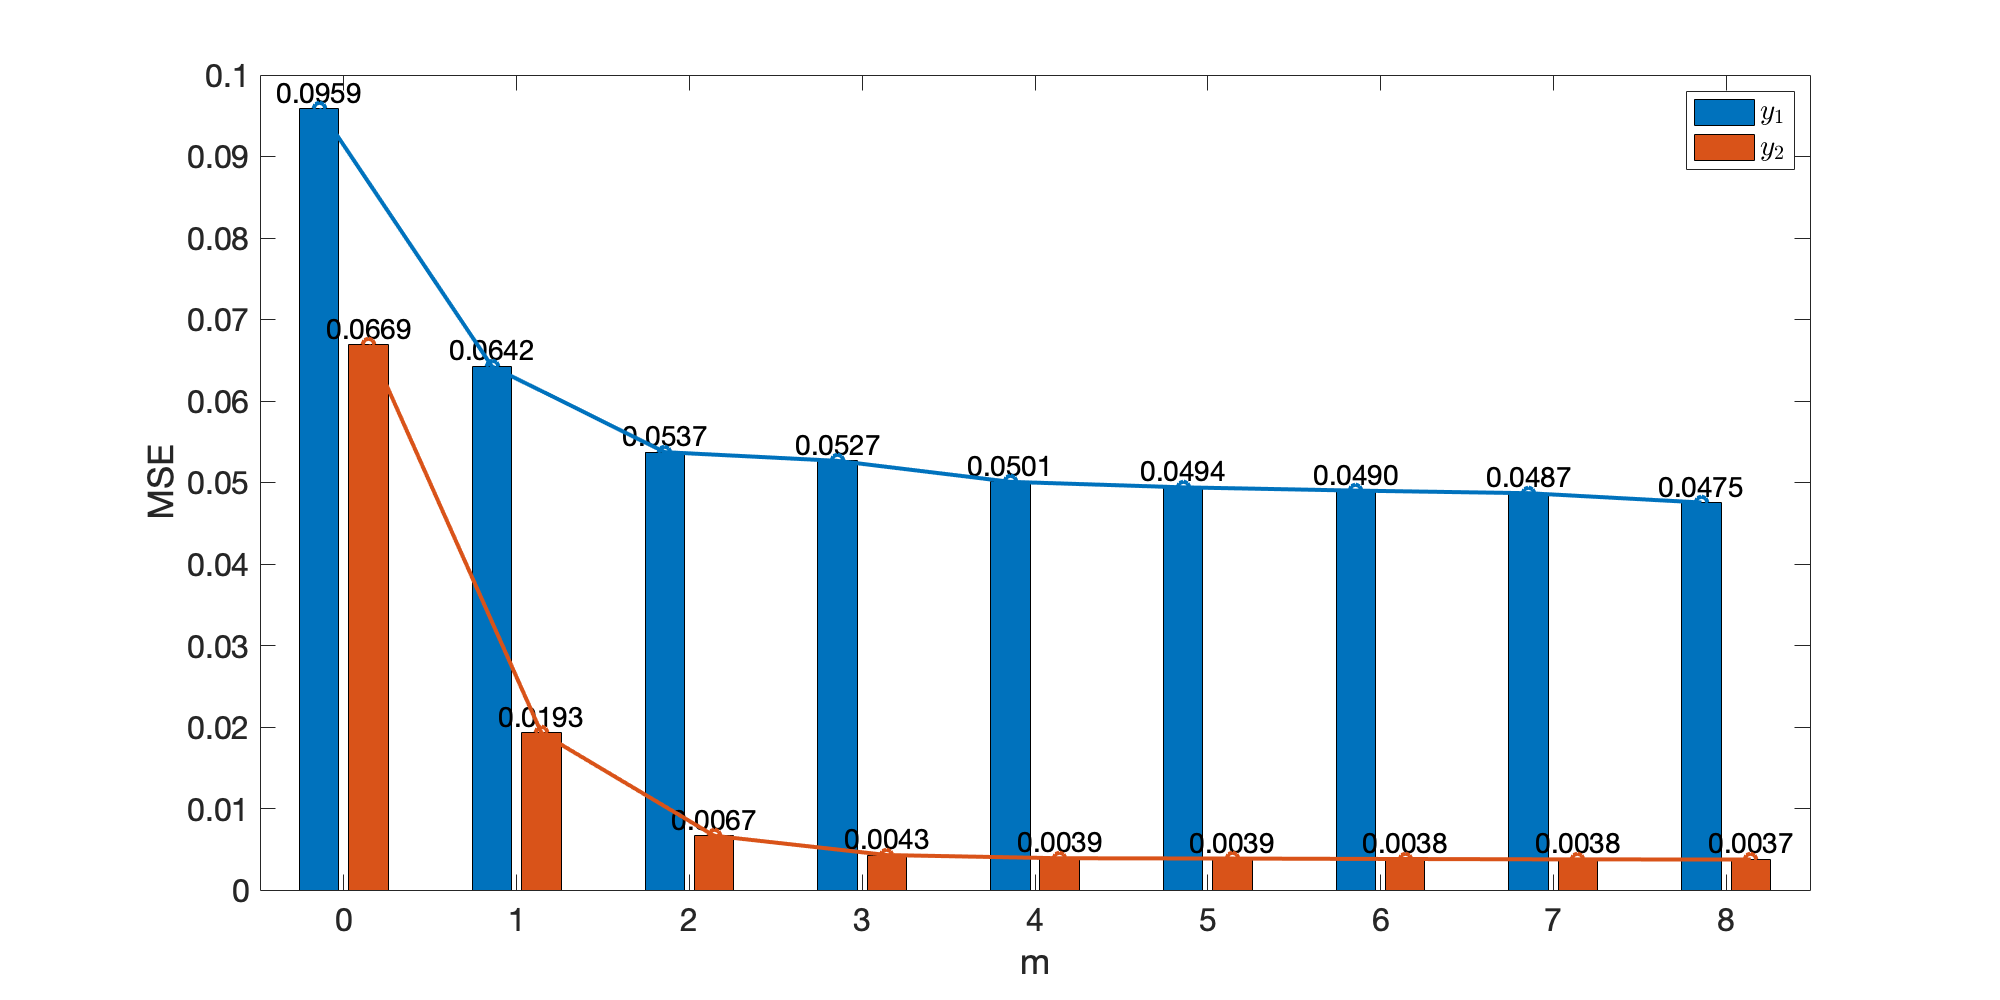
\includegraphics[width=0.8\textwidth]{m_mse.png}
        \vspace{-0.5cm}
        \caption{MSEs of different $m$th polynomial curve on dataset $y_1$ and $y_2$. $m$ is the polynomial degree.}
        \label{fig:1}
    \end{figure}

    \subsection{2nd polynomial vs log-transformed Linear Regression}
    The log-transformed linear regression seems to be more sensitive to the noise. For $y_1$ in large noise, its MSE of the fitting curve is 0.0747, even larger than 1st polynomial (0.0642) and best 2nd polynomial (0.0537). But for $y_2$, its MSE is 0.0069, which is comparable with 2nd polynomial (0.0067) and much lower than 1st polynomial (0.0193). This situation also meets the curves performance as shown in Fig. ~\ref{fig:2}. Therefore, when data has less noise, we are able to use only 2 parameters, bias and 1st degree coefficient, to model the curve, without the extra $t^2$ term, increasing the model robustness and reduce overfitting risks. 

    \makeatletter
    \setlength{\@fptop}{0pt}
    \makeatother
    \begin{figure}[t!]
        \centering
        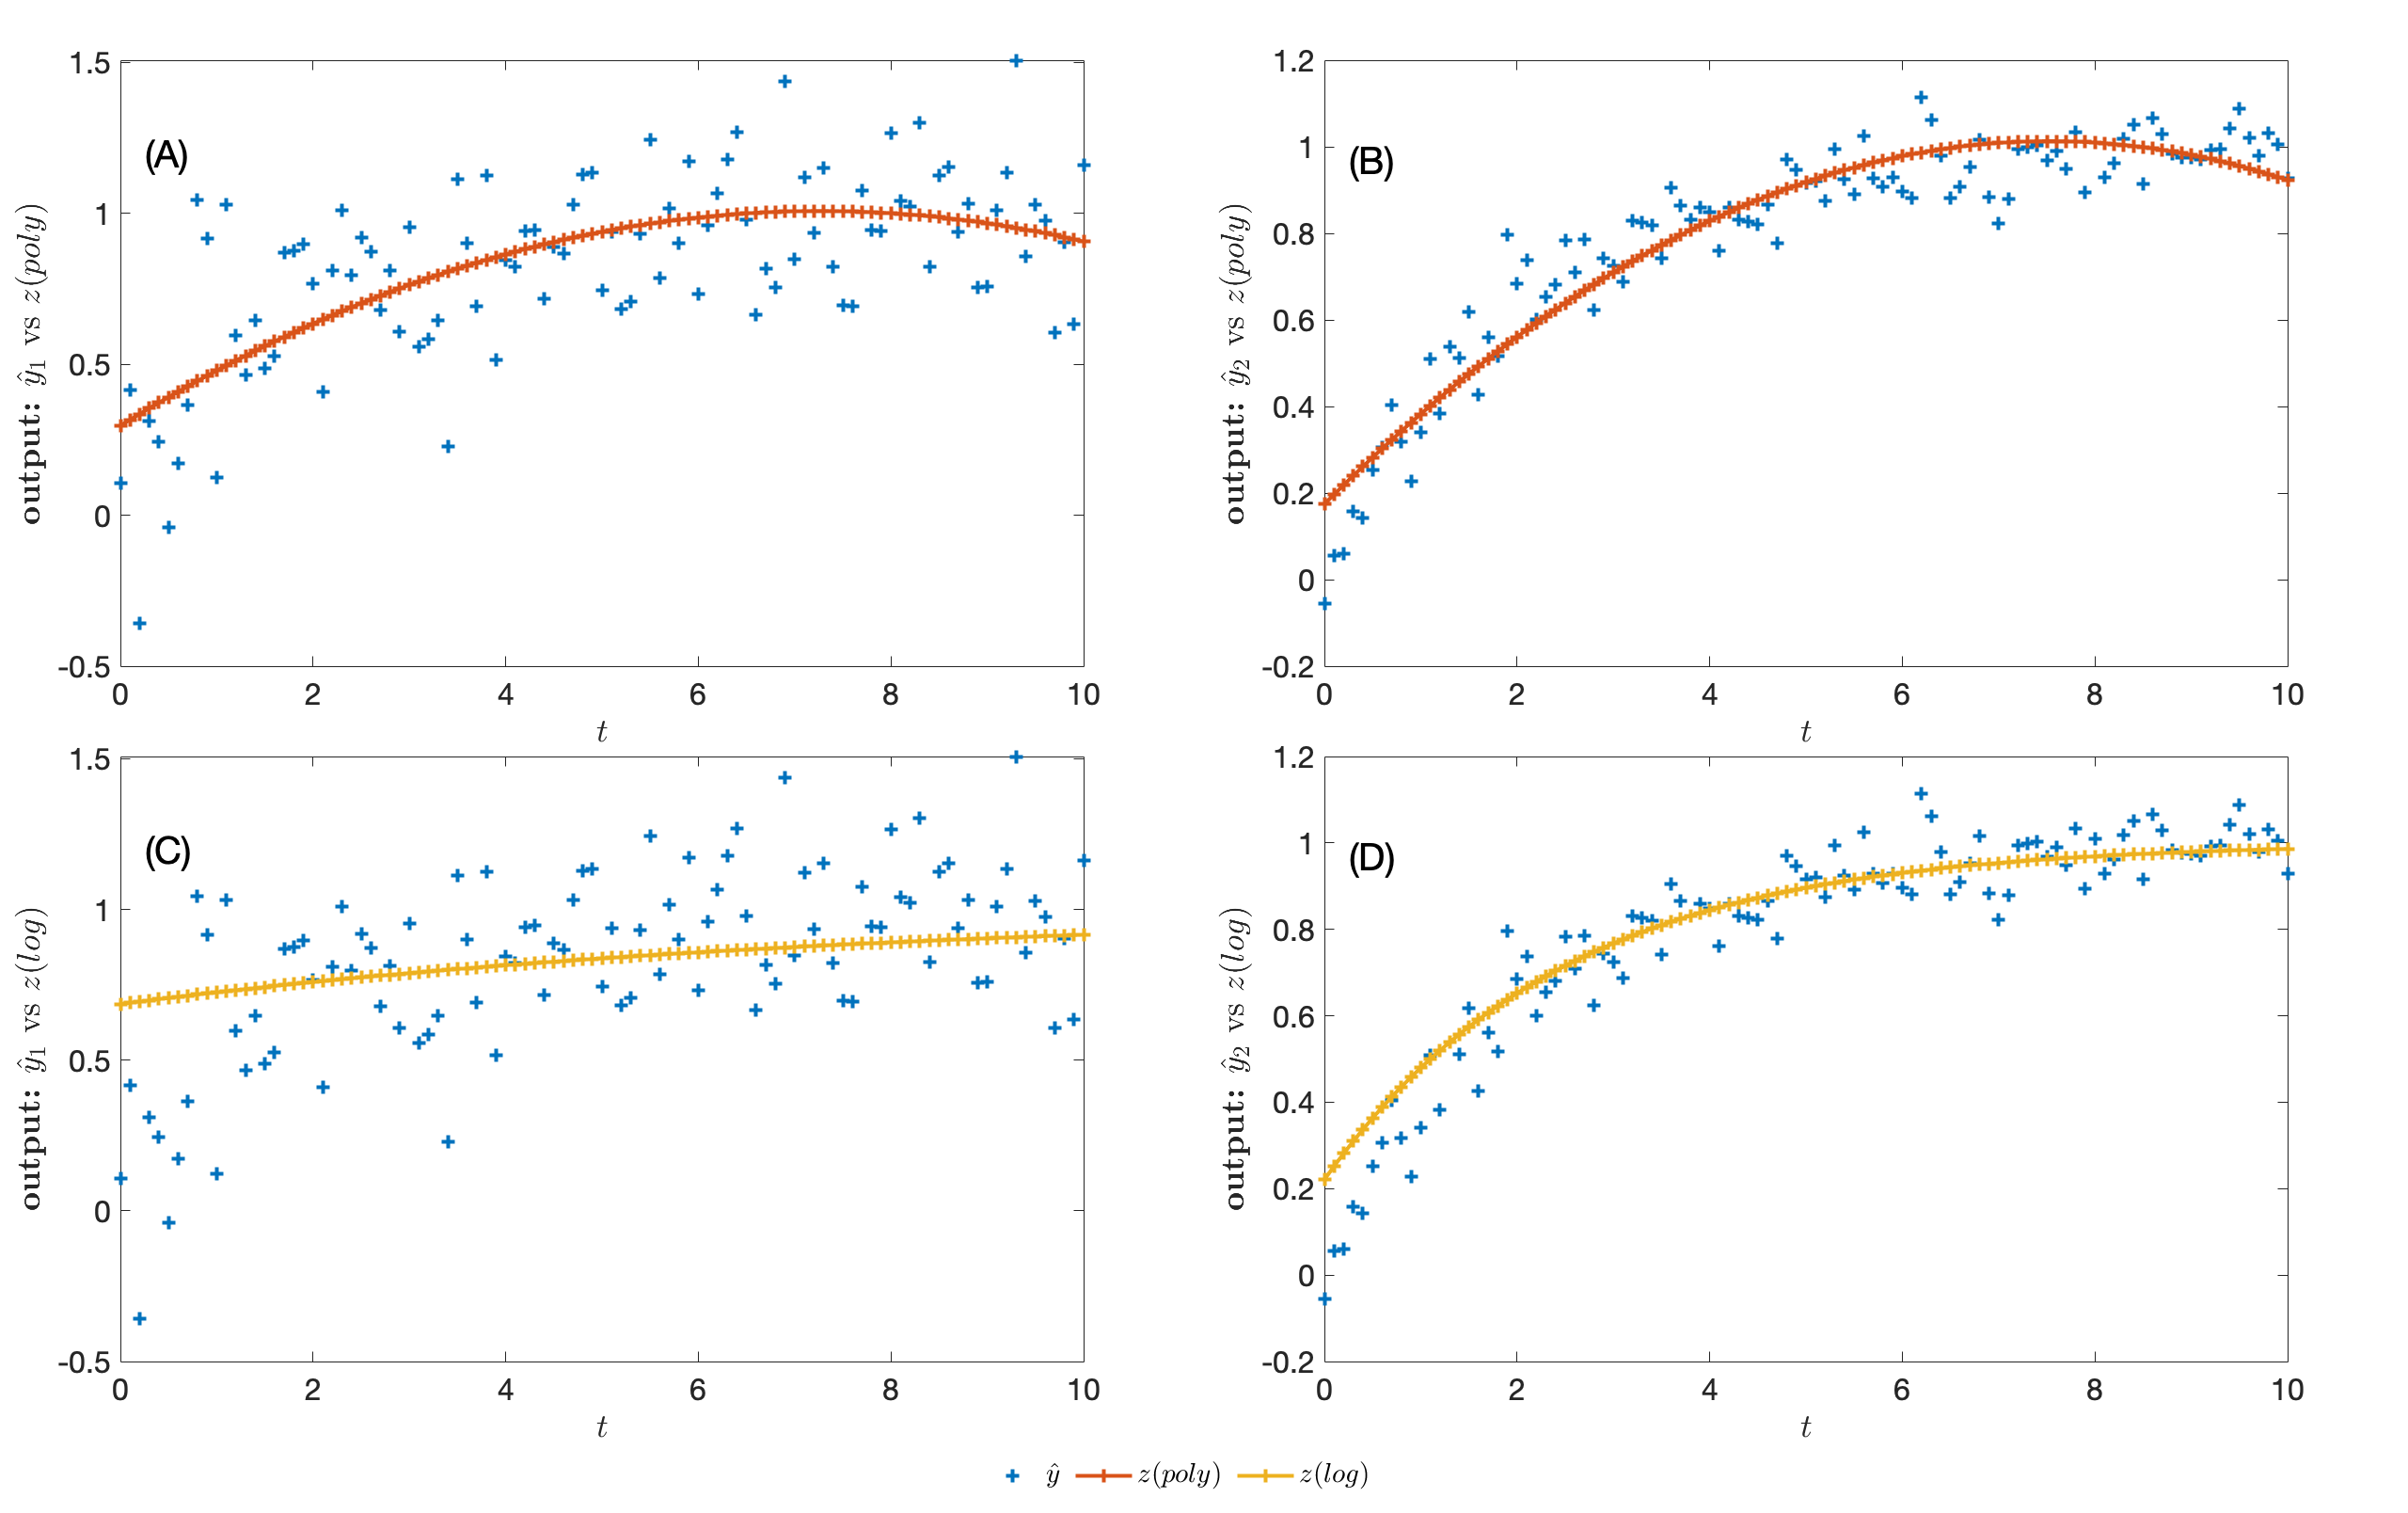
\includegraphics[width=0.8\textwidth]{m2_log_fit.png}
        \vspace{-0.5cm}
        \caption{Fitting curves of 2nd polynomial and log-transformed linear regression. (A)(B): 2nd polynomial curve on $y_1$ and $y_2$; (C)(D): log-transformed linear regression curve on $y_1$ and $y_2$}
        \label{fig:2}
    \end{figure}

    \section{Conclusion}
    Based on the results in Section 3, our choice of the best \textbf{m} would change based on different prerequisites:
    \begin{itemize}
    \item If measurements are only generated by current methods and all datasets are valid, we would choose $m=2$, 2nd polynomial as the optimal measurement function, since it would fit data best, reducing about 27\% MSE when using fitting approach (b). 
    \item If measurement is not limited to current methods or data with large noise could be removed (like $y_1$), we would choose $m=1$, the log-transformed linear regression as the measurement function, because it could fit clean data well together with fewer model parameters. Fewer parameters could reduce the overfitting risk so as to improve potential performance when applying it on different datasets. 
    \end{itemize}
\end{document}